%!TEX root = practicum4.tex
The display method \t{display_circumscribed_circles}, see \autoref{lst:a:display_circumscribed_circles}, draws the Delaunay Triangulation and the circumscribed circles of three randomly chosen circles. To run the script \t{assignment4A} with this display method use the flag \t{circ}, the result of one such call is shown in \autoref{fig:b:circles}.

\lstinputlisting[linerange={157-158, 160-160, 168-168, 176-186}, label={lst:a:display_circumscribed_circles}, caption={The relevant part of the method \t{display_circumscribed_circles()}.}]{../assignment4a.py}

Circles are drawn with the provided method \t{draw_circle} which expects the centre and the radius of circle. The centre of the circle through all three points of a triangle is the circumcentre of the triangle, which is stored in the object \t{Face}.

To determine the radius of a circle we compute the distance between one of the points, i.e. the origin of the outer component of the face, on the circle, the vertices of the triangle, and its centre.

\begin{figure}
	\centering
	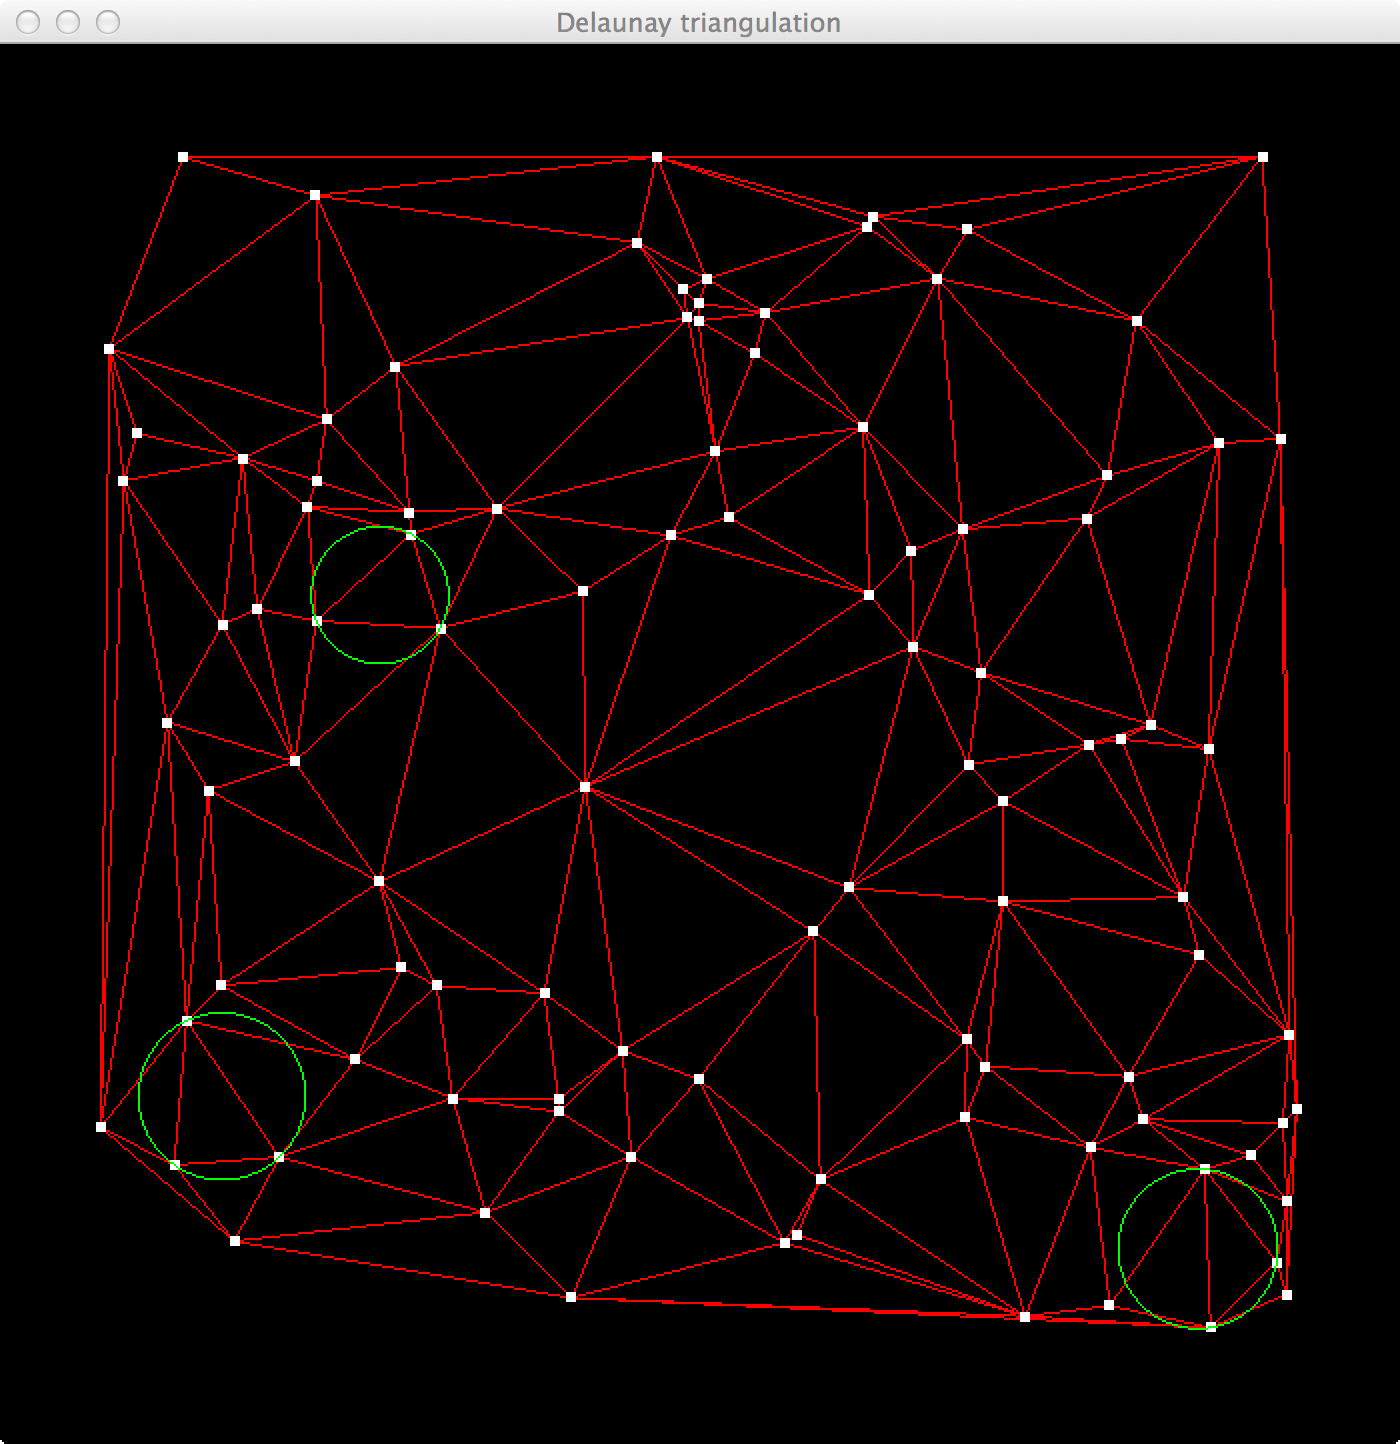
\includegraphics[width=0.405\textwidth]{./img/b_circles}
	\caption{The Delaunay triangulation of the white points is shown in red, the circumscribed circles of three randomly selected triangles is shown in green.}
	\label{fig:b:circles}
\end{figure}